\chapter{Discussão de resultados}

\par Neste capítulo serão apresentados e discutidos os resultados obtidos pela pesquisa e implementação 
do sistema de otimização do processo de fabricação de calças. Tal discussão será realizada em forma de
casos de teste, buscando demonstrar o comportamento do algoritmo genético de diferentes formas.

\par Desde o princípio, quando começou-se a discutir sobre o tema do 
trabalho de conclusão de curso, teve-se a ideia de desenvolver algo relacionado
à inteligência artificial, por ser um assunto de bastante relevância na área de desenvolvimento de software. 
Dentro desse campo então, realizando algumas buscas na internet, foi encontrado
o assunto de algoritmos genéticos.
Coincidentemente foi lecionada, no primeiro semestre deste ano, a disciplina
"sistemas especialistas", na qual o assunto foi abordado, o que facilitou bastante o aprendizado.

\par Assim, como sugestão do professor orientador, foi decidido então
desenvolver uma aplicação para otimizar um processo de distribuição de atividades entre
costureiras para um microempresário da cidade de Cachoeira de Minas - MG, do ramo de costura. Constatamos 
que um sistema \textit{web} seria mais cômodo de ser utilizado, por não precisar de
nenhuma instalação por parte do usuário e ainda poder ser acessado de qualquer lugar, desde que estivesse 
conectado à internet.

\par Assim sendo, foram adotadas como tecnologias para o desenvolvimento em
plataforma Web os \textit{frameworks} JSF e Primefaces. Além disso, foi utilizado
um \textit{plug-in} denominado \texttt{JBoss Tools}, o qual foi de grande utilidade
para gerar as classes modelos a partir do banco de dados.

\par Inicialmente foi tomado como base o caso do microempresário citado acima,
todavia, logo após iniciarmos o trabalho, o proprietário fez uma reestruturação de processos em sua empresa. 
Portanto, sua maneira de trabalhar deixou de ser um cenário no qual algoritmos genéticos
pudessem ser aplicados, consequentemente, fechou-se um escopo para que o trabalho
pudesse continuar, conforme descrito na seção 3.3.2 do quadro metodológico. Com
o escopo definido, o foco passou a ser na definição da estrutura dos elementos do algoritmo genético.


\par Posto isso, seguindo os passos descritos no quadro metodológico, foi obtido como resultado a aplicação
capaz de distribuir atividades de forma a se obter o menor custo e o menor tempo de produção, 
alcançando assim os objetivos específicos. Com a aplicação finalizada, foram realizados então casos de 
testes, a fim de colocar em prova a eficiência da ferramenta para se buscar melhores soluções nas distribuição 
de tarefas, conforme mostram as seções seguintes.


\section{Teste considerando somente o tempo de produção}

\par Este teste demonstra a distribuição de lotes levando em consideração o
tempo de cada costureira para fabricação das peças. Nesse teste será definido o
preço por peça igual para as costureiras, alterando somente o tempo por peça de
cada uma. Para esse teste foi cadastrado um processo de produção informando o
cliente, o modelo da calça e a data e hora da entrega conforme mostra a Figura~\ref{fig:cad_processo1}.

\begin{figure}[h!]
	\centerline{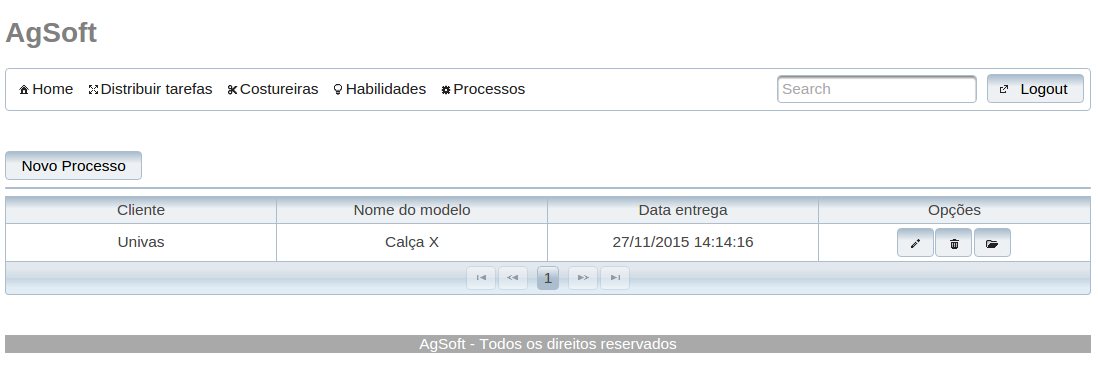
\includegraphics[width=14.7cm]{./imagens/teste_processo.png}}
	\caption[Criação de um processo.]
	{Criação de um processo. \textbf{Fonte:} Desenvolvido pelos autores.}
	\label{fig:cad_processo1}
\end{figure}

\par Todo processo ao ser criado, por padrão já contém as atividades principais
 Carimbo e Finalização, conforme mostra a Figura~\ref{fig:processo_cadastrado}.


\begin{figure}[h!]
	\centerline{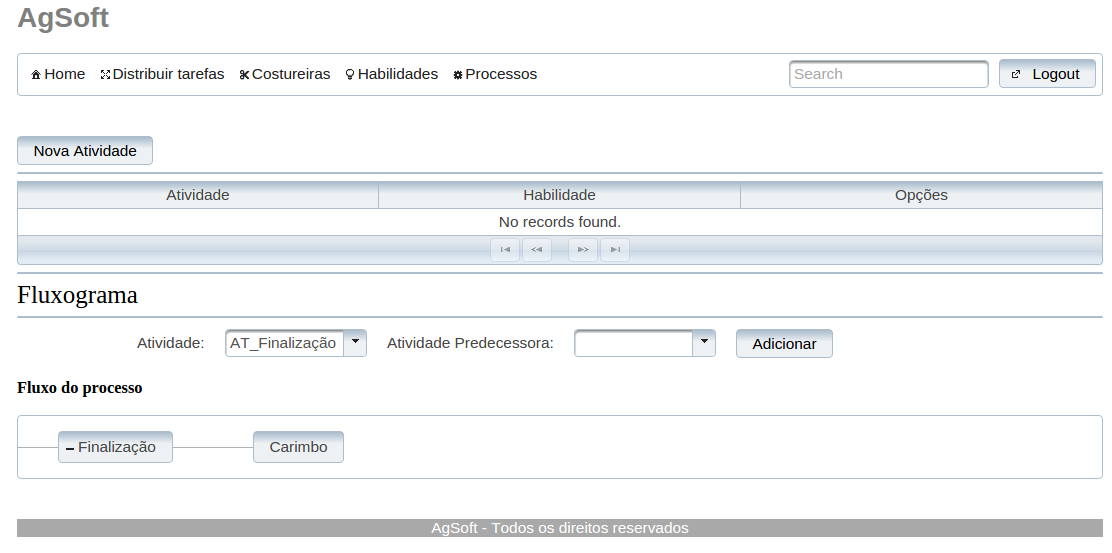
\includegraphics[width=13cm]{./imagens/tela_processo_teste1.png}}
	\caption[Detalhes do processo cadastrado.]
	{Detalhes do processo cadastrado. \textbf{Fonte:} Desenvolvido pelos autores.}
	\label{fig:processo_cadastrado}
\end{figure}

\par Após a criação do processo, foram definidas quais costureiras possuem a
habilidade para realizar as atividades que compõem o processo, sendo definidas
para realizar a atividade finalização, as costureiras Maria e Duda, ambas cobram o 
mesmo valor por peça, porém, o tempo gasto para fabricar uma peça é diferente, 
conforme mostra a Figura~\ref{fig:costureira_habilidade}. Vale ressaltar que
a atividade carimbo é realizada somente pelo proprietário da fábrica, pois é a
atividade em que serão distribuídas as peças para serem produzidas. 


\begin{figure}[h!]
	\centerline{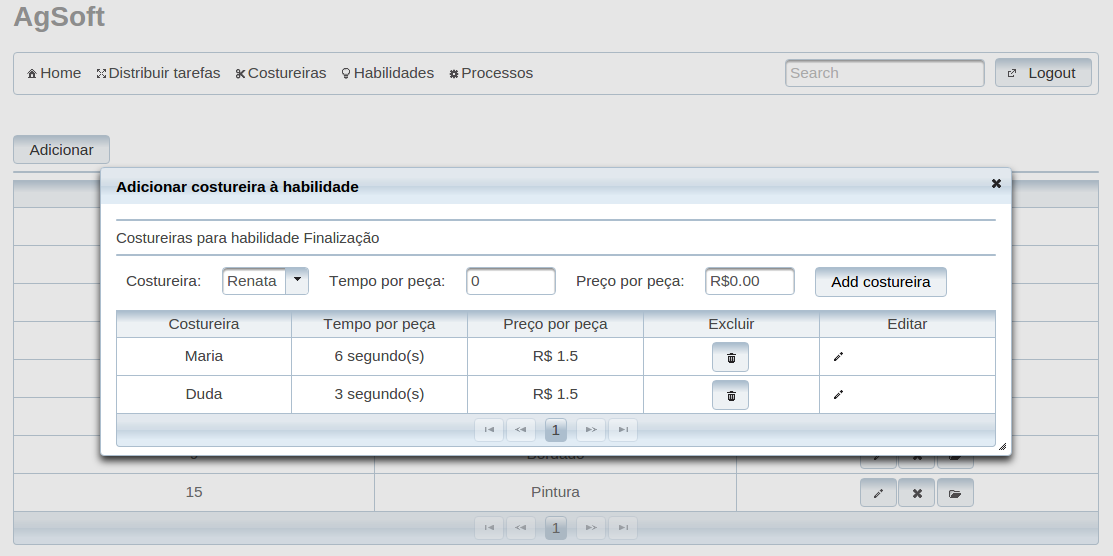
\includegraphics[width=14.7cm]{./imagens/tela_habilidade_teste1.png}}
	\caption[Inserindo costureiras na habilidade Finalização.]
	{Inserindo costureiras na habilidade Finalização. \textbf{Fonte:} Desenvolvido
	pelos autores.}
	\label{fig:costureira_habilidade}
\end{figure}


\par Feito isso, foi aberto o processo para a distribuição
das atividades, através do menu "Distribuição de Tarefas".
Ao acessar a página todos os processos criados são
listados, como mostra a Figura~\ref{fig:distribuicao_tarefas}:

\begin{figure}[h!]
	\centerline{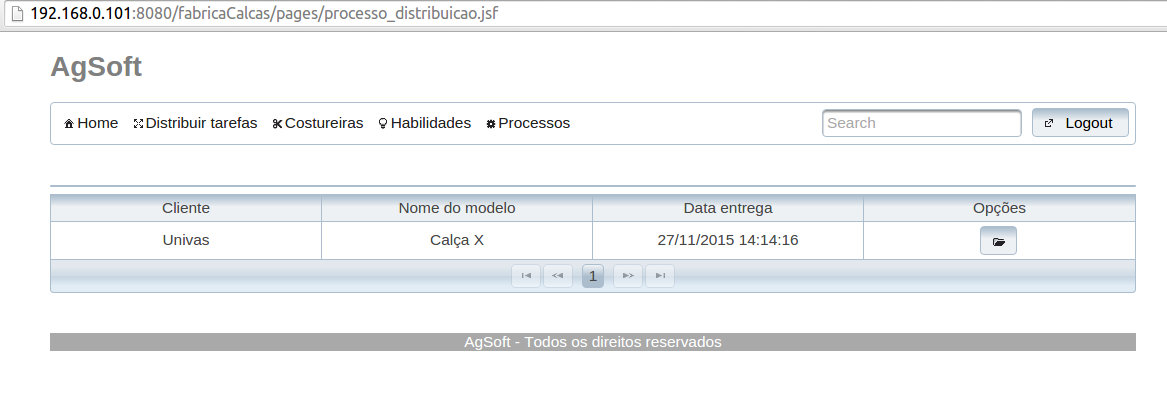
\includegraphics[width=14.7cm]{./imagens/tela_distribuicao_tarefas.png}}
	\caption[Tela de distribuição de tarefas.]
	{Tela de dritribuição de tarefas. \textbf{Fonte:} Desenvolvido
	pelos autores.}
	\label{fig:distribuicao_tarefas}
\end{figure}


\par Ao clicar no botão "Abrir" da coluna opções é mostrada a tela para que o
usuário insira os dados como número de peças, total de peças por lote e data de
início. Depois de inseridos os dados, ao clicar no botão "Iniciar Distribuição", o sistema executa
o algoritmo genético e retorna para o usuário a melhor solução
encontrada com base nos dados inseridos, conforme mostra a
Figura~\ref{fig:resultado_distribuicao_teste1}.

\begin{figure}[h!]
	\centerline{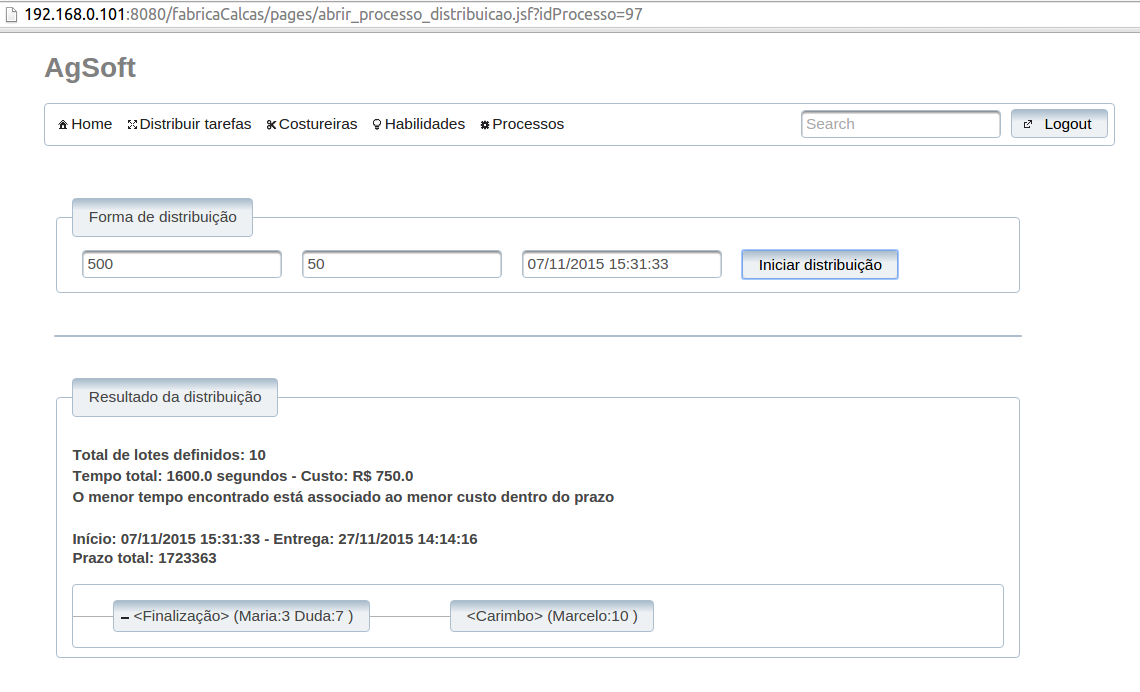
\includegraphics[width=14.7cm]{./imagens/resultado_distribuicao_teste1.png}}
	\caption[Resultado da distribuição de lotes considerando o tempo de produção.]
	{Resultado da distribuição de lotes considerando o tempo de produção. \textbf{Fonte:} Desenvolvido pelos
	autores.}
	\label{fig:resultado_distribuicao_teste1}
\end{figure}

\par Os valores então foram definidos, a distribuição foi realizada e o resultado apresentado. 
Conforme ilustrado na Figura~\ref{fig:costureira_habilidade}, Maria possui
o tempo de produção maior que Duda, por isso ela recebeu um número menor de lotes
para produzir, conforme ilustrado na
Figura~\ref{fig:resultado_distribuicao_teste1}.

\par Se o tempo de cada costureira for alterado, um novo resultado será
retornado, levando em consideração as alterações. Para isso, foi definido para
Maria o tempo de 4 segundos e para Duda o tempo de 7 segundos, conforme ilustra
a Figura~\ref{fig:tempo_costureiras}. 

\newpage

\begin{figure}[h!]
	\centerline{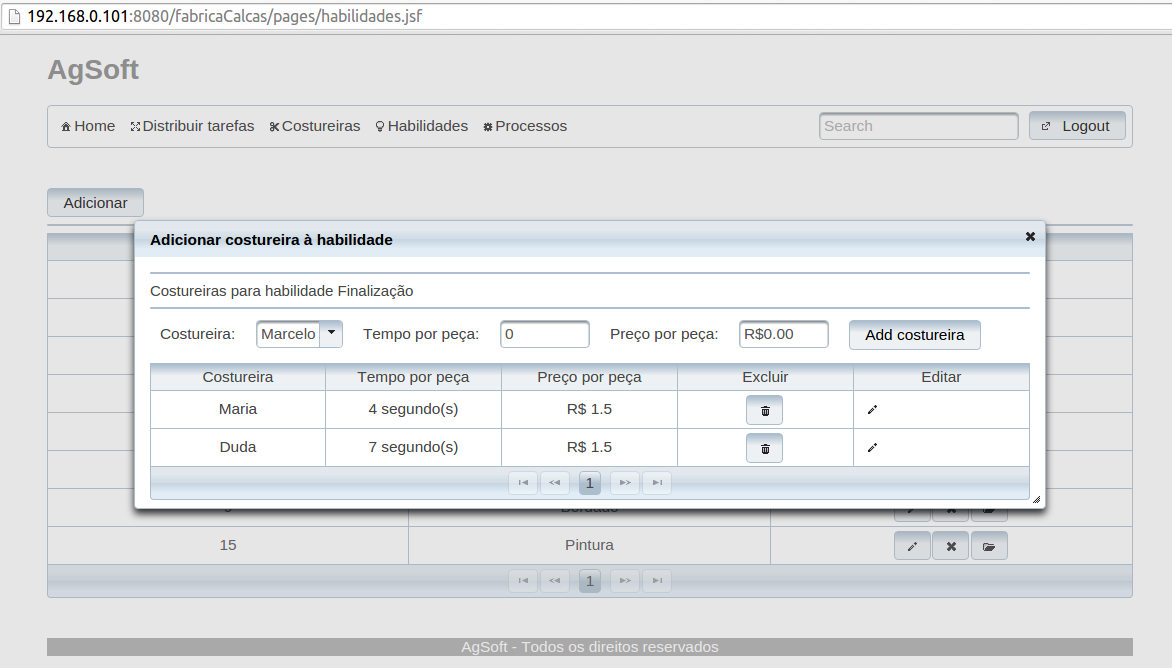
\includegraphics[width=14cm]{./imagens/alterando_tempo_costureira.png}}
	\caption[Alteração no tempo de produção entre as costureiras.]
	{Alteração no tempo de produção entre as costureiras. \textbf{Fonte:}
	Desenvolvido pelos autores.}
	\label{fig:tempo_costureiras}
\end{figure}

\par Após executar novamente a distribuição, foi retornado um novo resultado
ilustrado na Figura~\ref{fig:novo_resultado_distribuicao_teste1}.



\begin{figure}[h!]
	\centerline{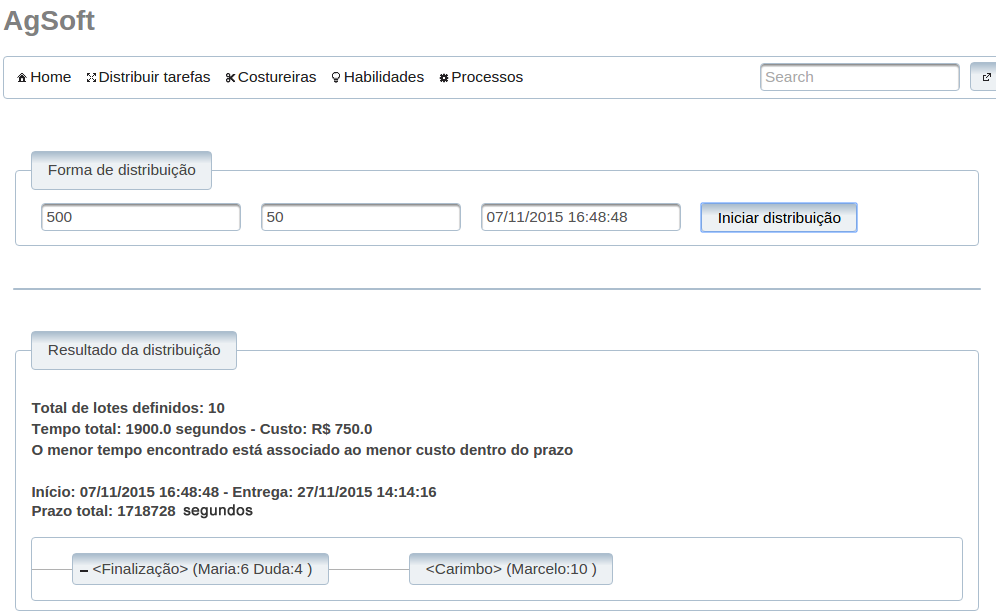
\includegraphics[width=14.7cm]{./imagens/novo_resultado_alterado_tempo_teste1.png}}
	\caption[Resultado da distribuição de lotes após a alteração do tempo de
	produção entre as costureiras.]
	{Resultado da distribuição de lotes após a alteração do tempo de
	produção entre as costureiras. \textbf{Fonte:} Desenvolvido pelos autores.}
	\label{fig:novo_resultado_distribuicao_teste1}
\end{figure}

\par Neste resultado, Maria obteve mais lotes que Duda para produzir, pois o seu
tempo de produção é menor.

\section{Teste considerando o custo de produção}

\par Este teste foi feito utilizando-se o mesmo processo do teste realizado na seção anterior,
porém foi definido o mesmo tempo de produção para ambas as costureiras,
alterando somente o custo. Foi definido o tempo de 5 segundos para as costureiras Maria e Duda e o preço por peça R\textdollar 1,50 e R\textdollar 
2,70, respectivamente. Além disso, foram definidos os mesmos valores X e Y
relativos à posição geográfica para Maria e Duda, de forma a manter o tempo de
transporte semelhante para ambas.
A Figura~\ref{fig:custo_entre_costureiras} mostra a definição de tempo e custo
para ambas as costureiras.

\begin{figure}[h!]
	\centerline{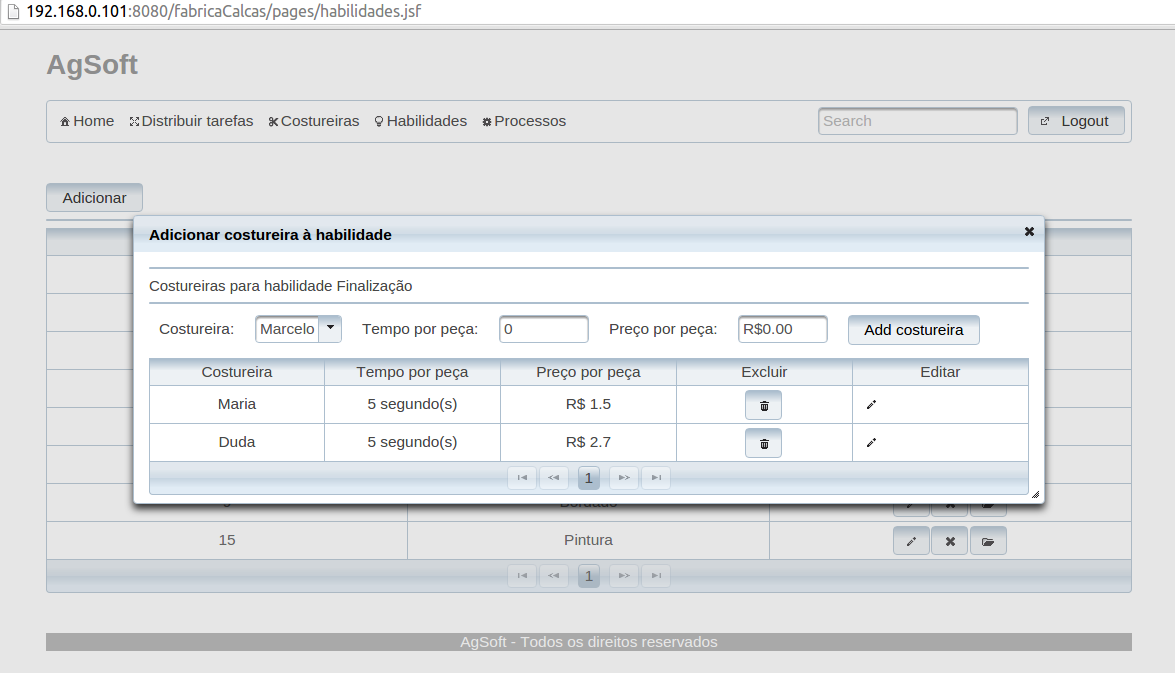
\includegraphics[width=14.7cm]{./imagens/custo_entre_costureiras_teste2.png}}
	\caption[Custo entre as costureiras da atividade Finalização.]
	{Custo entre as costureiras da atividade Finalização. \textbf{Fonte:}
	Desenvolvido pelos autores.}
	\label{fig:custo_entre_costureiras}
\end{figure}

\par Ao executar a distribuição, é retornado o seguinte resultado, ilustrado na
Figura~\ref{fig:resultado_custo}.



\begin{figure}[h!]
	\centerline{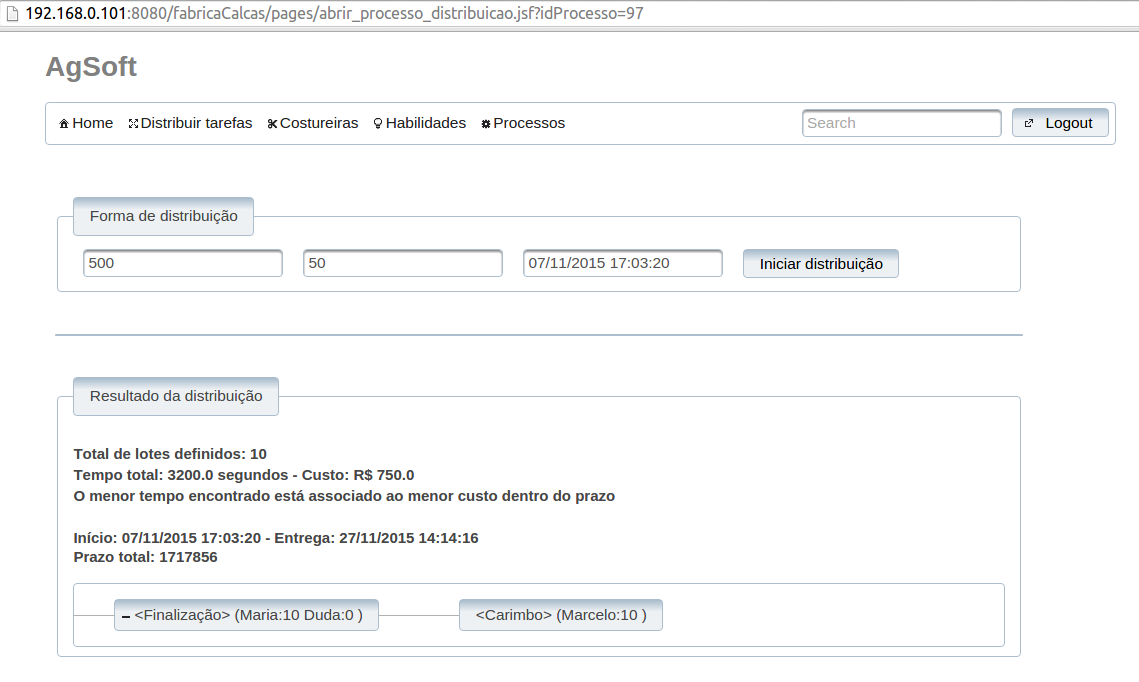
\includegraphics[width=13cm]{./imagens/resultado_teste2.png}}
	\caption[Resultado da distribuição de lotes considerando o custo.]
	{Resultado da distribuição de lotes considerando o custo. \textbf{Fonte:}
	Desenvolvido pelos autores.}
	\label{fig:resultado_custo}
\end{figure}

\par Com base no resultado obtido, o algoritmo decidiu que, pelo fato de
Maria e Duda obterem o mesmo tempo de produção e Duda ter um preço por peça
bem superior que o de Maria, Duda não deve receber nenhum lote para produzir, pois neste
caso é possível que Maria produza sozinha os lotes dentro do prazo de entrega do
processo. Caso Maria não conseguisse produzir os lotes no prazo estipulado, o
algoritmo adequaria a distribuição distribuindo alguns lotes para Duda para
conseguir alcançar o prazo de entrega, todavia, fazendo isso, o custo tende a
aumentar, esse caso será mostrado com mais detalhes na seção 4.3.

\par Caso Maria e Duda gastassem o mesmo tempo, cobrassem o mesmo preço e o tempo de
transporte das peças entre todos os envolvidos no processo fosse o mesmo para ambas, 
o algoritmo distribuiria lotes para Duda, pois, mesmo a costureira Maria
conseguindo fabricar as peças dentro do prazo, nesse caso, se Duda recebesse
alguns lotes para produzir, isso não interferiria no preço final e a produção
seria realizada em um tempo menor, como mostra a
Figura~\ref{fig:resultado_tudo_igual}.

\begin{figure}[h!]
	\centerline{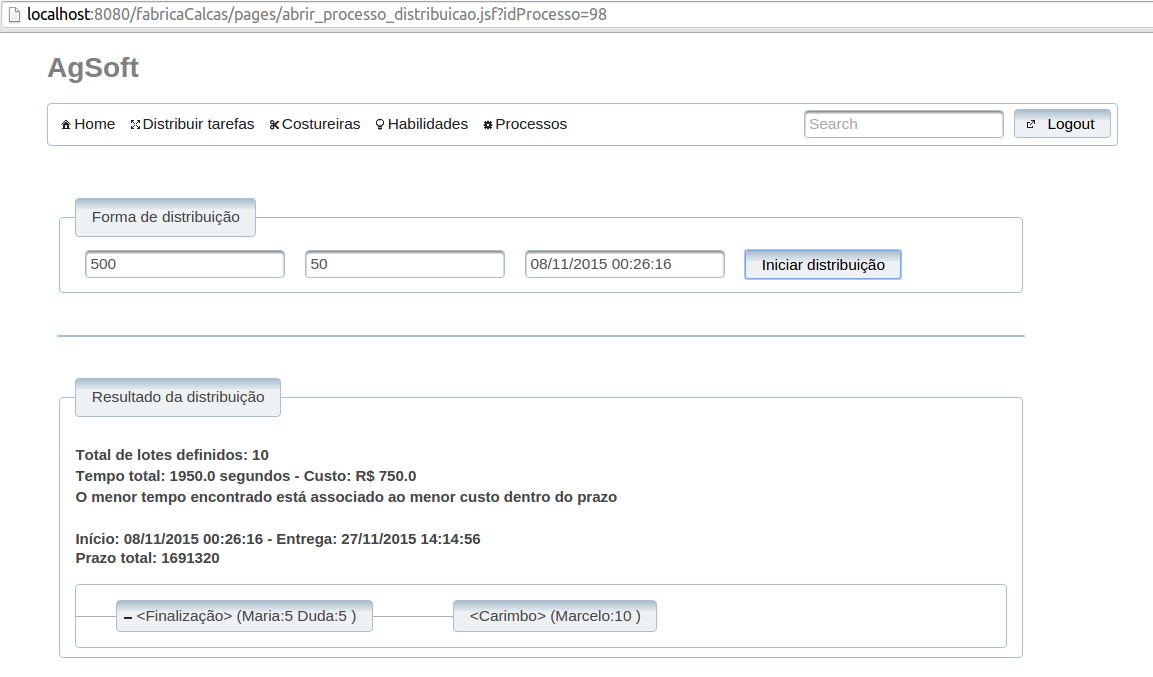
\includegraphics[width=14.7cm]{./imagens/resultado_tudo_igual_teste2.png}}
	\caption[Resultado da distribuição de lotes com configurações iguais entre as
	costureiras.] 
	{Resultado da distribuição de lotes com configurações iguais entre as
	costureiras. \textbf{Fonte:}
	Desenvolvido pelos autores.}
	\label{fig:resultado_tudo_igual}
\end{figure}

\section{Teste considerando tempo x custo x prazo de entrega}

\par Este teste foi realizado para demonstrar a distribuição considerando o tempo de
produção, o custo e o prazo de entrega, assim, mesmo que uma costureira seja
inviável quanto ao custo, ela poderá receber lotes para produzir para que seja cumprido o prazo 
de entrega. Para isso as costureiras que possuem a habilidade finalização
ficarão com as seguintes configurações, como ilustra a
Figura~\ref{fig:configuracao_habilidade_costureira_teste3}.

\begin{figure}[h!]
	\centerline{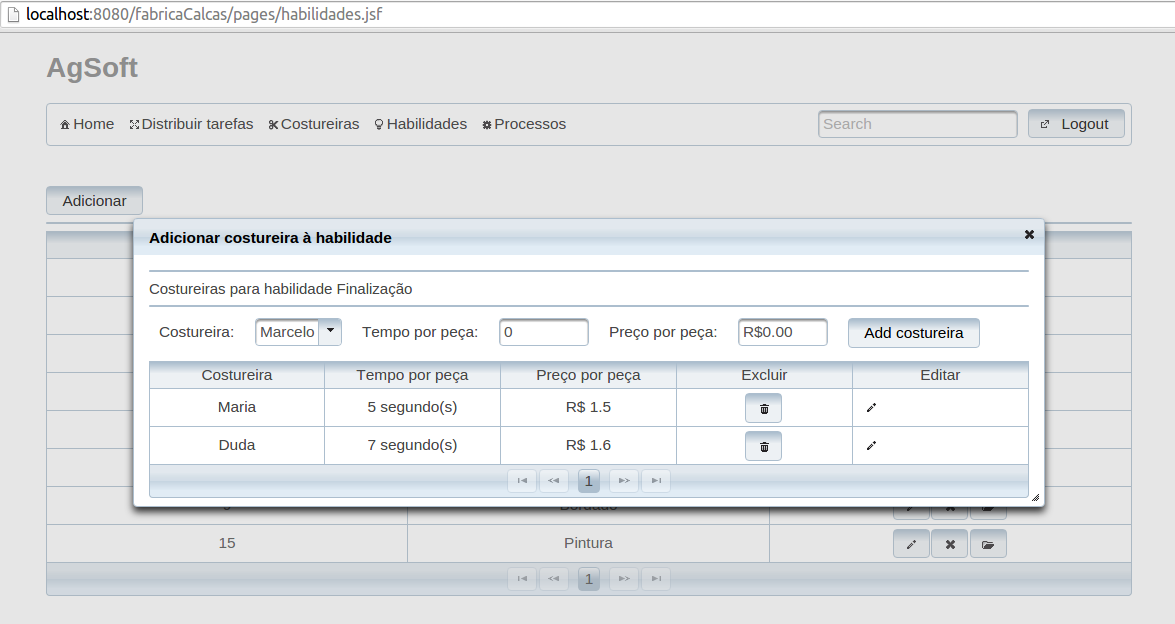
\includegraphics[width=14.7cm]{./imagens/cofiguracao_habilidade_teste3.png}}
	\caption[Configuração das costureiras da atividade Finalização.]
	{Configuração das costureiras da atividade Finalização. \textbf{Fonte:}
	Desenvolvido pelos autores.}
	\label{fig:configuracao_habilidade_costureira_teste3}
\end{figure}


\par A Figura~\ref{fig:resultado1_teste3} mostra o resultado da distribuição
com base nas configurações da habilidade Finalização, mostrada na
Figura~\ref{fig:configuracao_habilidade_costureira_teste3}.

\begin{figure}[h!]
	\centerline{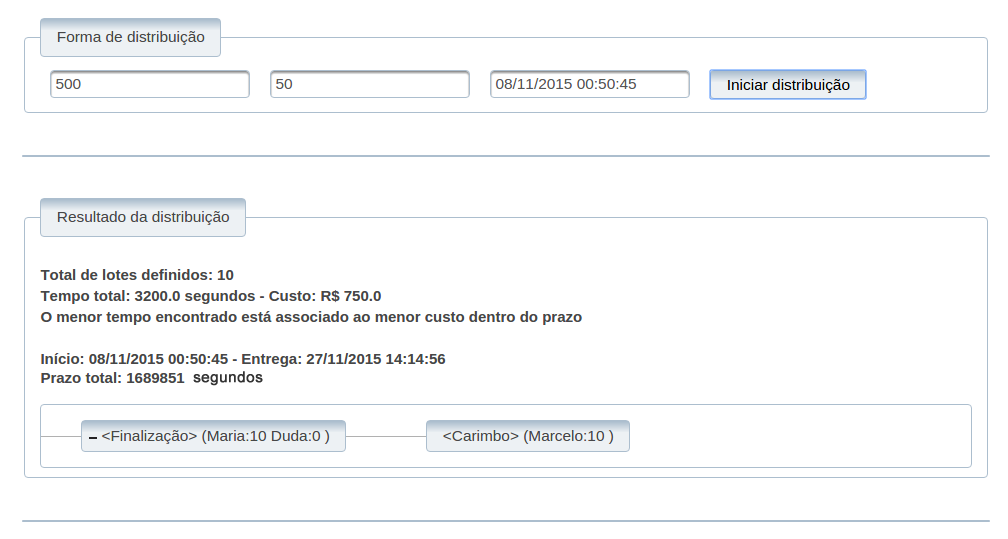
\includegraphics[width=13cm]{./imagens/resultado1_teste3.png}}
	\caption[Resultado da distribuição de lotes com prazo longo.]
	{Resultado da distribuição de lotes com prazo longo. \textbf{Fonte:} Desenvolvido pelos
	autores.}
	\label{fig:resultado1_teste3}
\end{figure}

\par Como ilustrado na Figura~\ref{fig:resultado1_teste3}, a costureira Duda
não recebeu nenhum lote, pois possui um tempo de produção e custo maior que
Maria e essa consegue cumprir o prazo de entrega, porém, caso Maria não
conseguisse atender o prazo, Duda poderia receber lotes para produzir mesmo que
o custo aumentasse.

A Figura~\ref{fig:resultado2_teste3} mostra a distribuição de lotes entre as
costureiras com a alteração na data de início do processo.

\begin{figure}[h!]
	\centerline{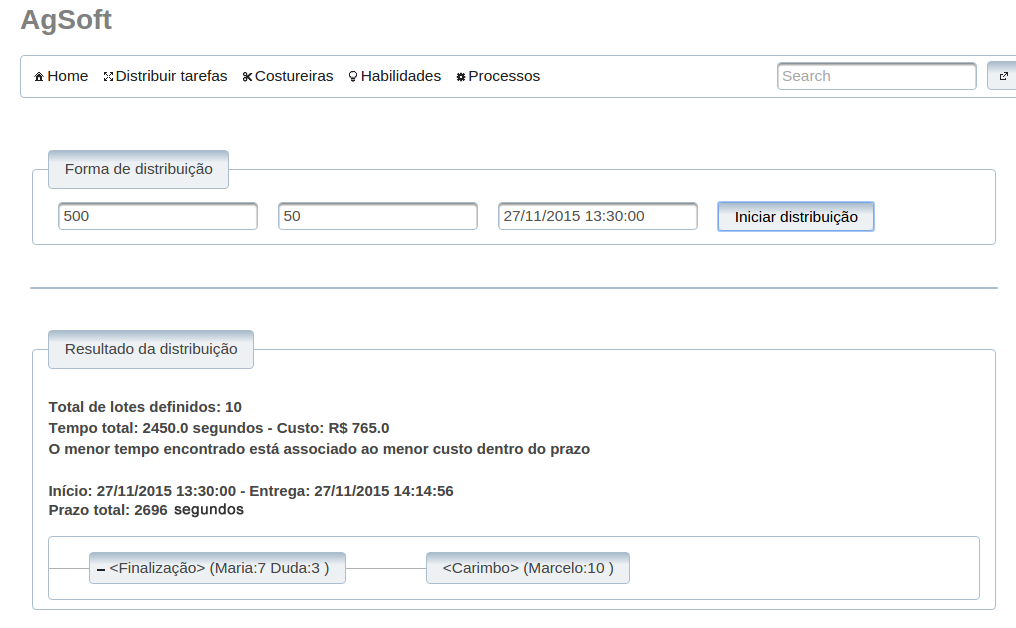
\includegraphics[width=14.7cm]{./imagens/resultado2_teste3.png}}
	\caption[Resultado da distribuição de lotes com prazo reduzido.]
	{Resultado da distribuição de lotes com prazo reduzido. \textbf{Fonte:} Desenvolvido pelos
	autores.}
	\label{fig:resultado2_teste3}
\end{figure}

\par Como ilustrado na Figura~\ref{fig:resultado2_teste3}, a costureira Duda
recebe 3 lotes para produzir, assim, o custo de produção aumenta com relação ao 
resultado da Figura~\ref{fig:resultado1_teste3}, porém o tempo de produção
diminui, sendo possível atender o prazo de entrega.


\section{Teste considerando o tempo de transporte}

\par Este teste foi realizado para demonstrar que mesmo as costureiras possuindo
o tempo e custo iguais, o tempo de transporte entre elas pode influenciar na distribuição dos lotes.

\par Para isso, foi necessário cadastrar um valor X e Y, correspondente às
coordenadas geográficas, para cada costureira, conforme mostra a Figura~\ref{fig:add_xy_costureira_teste4}.


\begin{figure}[h!]
	\centerline{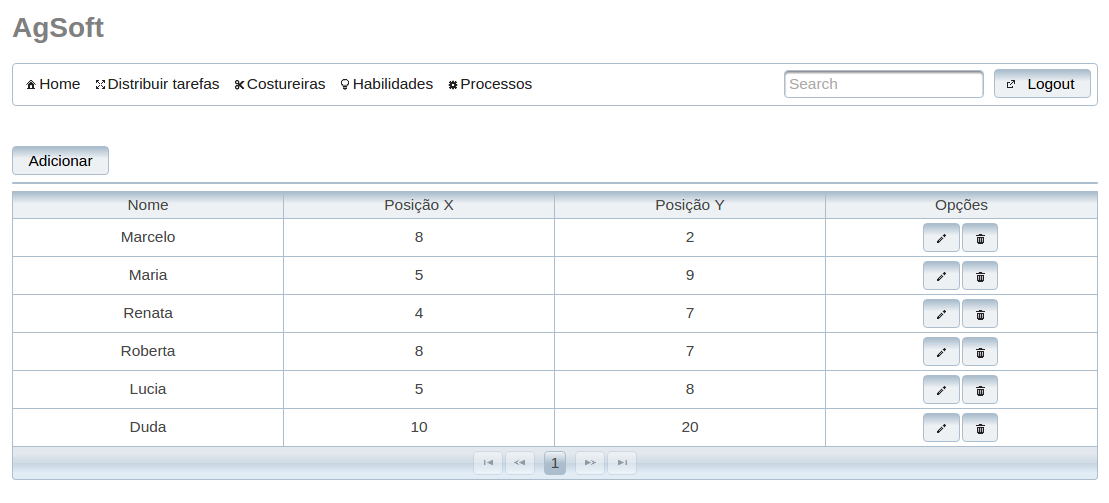
\includegraphics[width=14.7cm]{./imagens/posicao_xy_costureiras_teste4.png}}
	\caption[Tela de cadastro de costureiras.]
	{Tela de cadastro de costureiras. \textbf{Fonte:} Desenvolvido pelos autores.}
	\label{fig:add_xy_costureira_teste4}
\end{figure}


\par Neste teste foi considerado apenas o tempo de transporte, logo, o tempo e o
preço de confecção por peça das costureiras da atividade finalização possuem o
mesmo valor, conforme mostra a Figura~\ref{fig:at_finalizacao_teste4}.


\begin{figure}[h!]
	\centerline{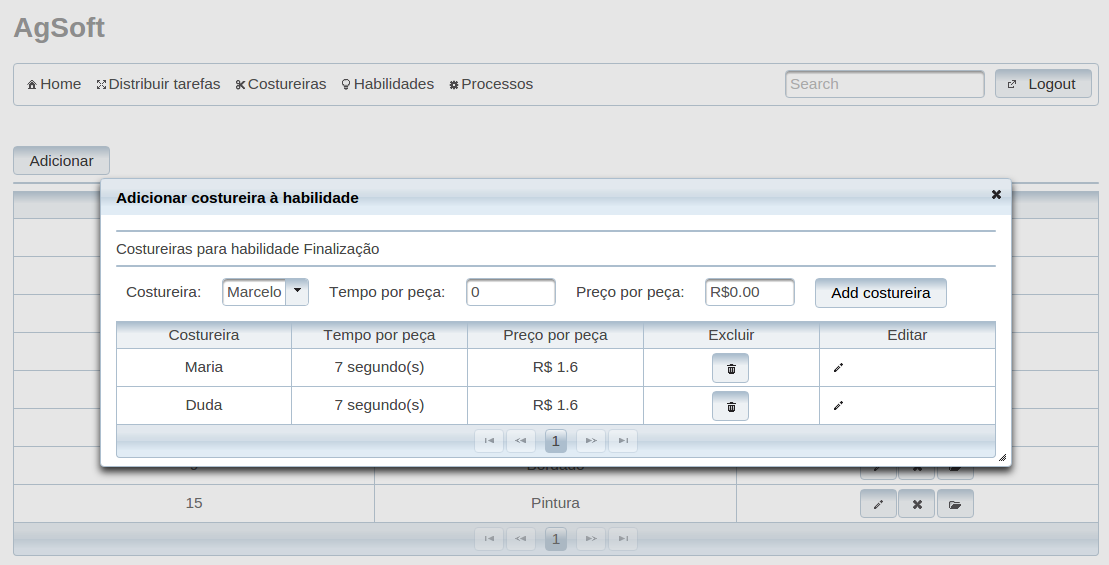
\includegraphics[width=14cm]{./imagens/cofig_at_finalizaca_teste4.png}}
	\caption[Configuração das costureiras da habilidade Finalização.]
	{Configuração das costureiras da habilidade Finalização \textbf{Fonte:}
	Desenvolvido pelos autores.}
	\label{fig:at_finalizacao_teste4}
\end{figure}



\par Feito isso, foi iniciado então o processo de distribuição das atividades,
através do menu "Distribuição de Tarefas". A Figura~\ref{fig:resultado_transporte_teste4} mostra o resultado obtido.

\newpage

\begin{figure}[h!]
	\centerline{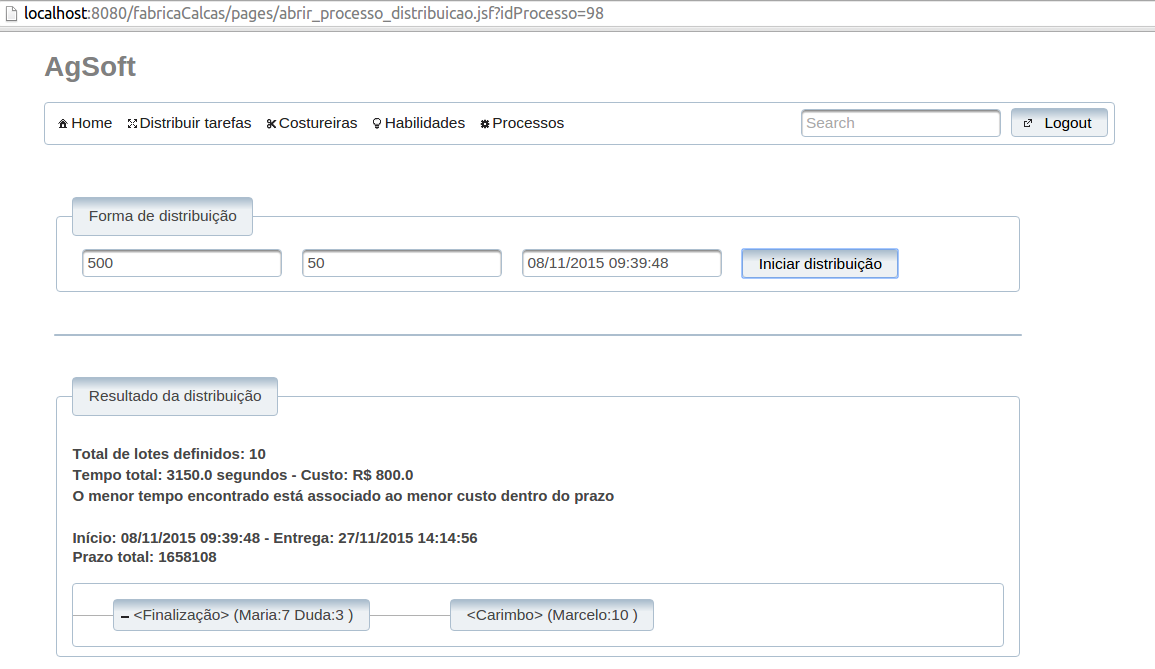
\includegraphics[width=14.7cm]{./imagens/resultado_transporte_teste4.png}}
	\caption[Resultado da distribuição de lotes considerando o tempo de transporte.]
	{Resultado da distribuição de lotes considerando o tempo de transporte. \textbf{Fonte:} Desenvolvido pelos
	autores.}
	\label{fig:resultado_transporte_teste4}
\end{figure}

\par Como mostrado na Figura~\ref{fig:add_xy_costureira_teste4}, a costureira
Duda fica mais distante do Marcelo e por isso recebe menos lotes para produzir em
relação à costureira Maria.

\par Para melhor ilustrar o tempo de envio das peças para as costureiras, na tela
de resultados há um detalhamento de todo cálculo realizado. A
Figura~\ref{fig:detalhameneto_transporte_teste4} mostra que o tempo de envio das peças para Duda é 
maior que o tempo de envio para Maria, comprovando o resultado mostrado na
Figura~\ref{fig:resultado_transporte_teste4}.

\begin{figure}[h!]
	\centerline{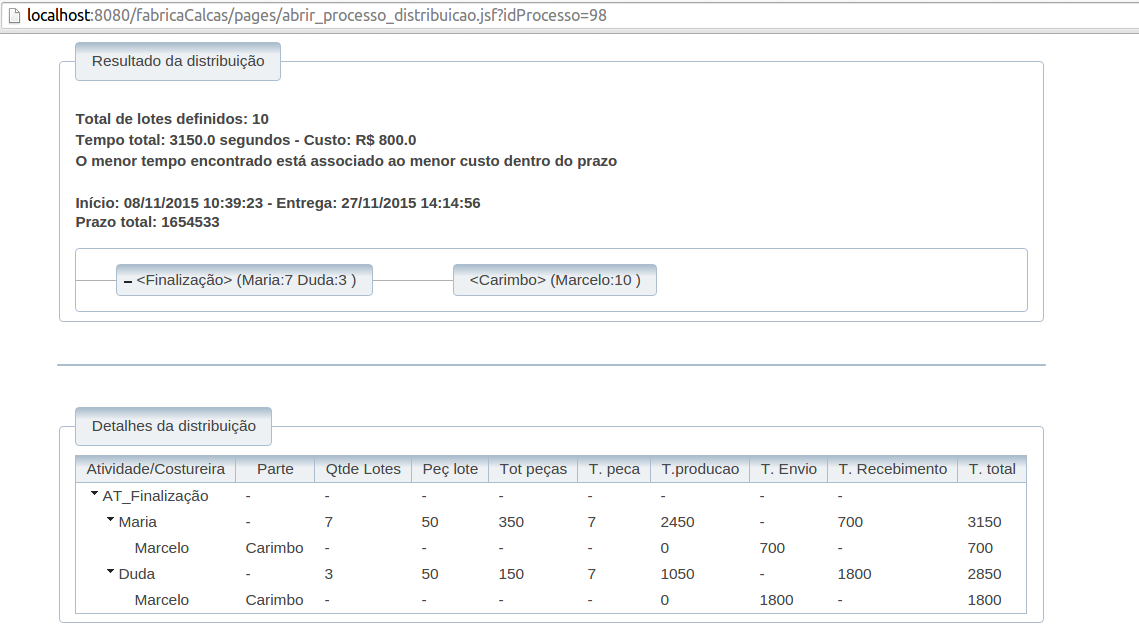
\includegraphics[width=13cm]{./imagens/detalhamento_transporte_teste4.png}}
	\caption[Distribuição das atividades.] 
	{Distribuição das atividades. \textbf{Fonte:} Desenvolvido pelos autores.}
	\label{fig:detalhameneto_transporte_teste4}
\end{figure}

\par Como mostrado na Figura~\ref{fig:detalhameneto_transporte_teste4}, o tempo
de envio das peças para Duda é 1800 segundos e para Maria 700, por isso
Duda recebe menos lotes para serem produzidos.


\section{Teste adicionando mais atividades ao processo}

\par Este teste foi realizado para demonstrar a adição de mais atividades no
processo e utiliza o mesmo processo da seção 4.1, porém será adicionado
à ele a atividade frente conforme mostra a Figura~\ref{fig:add_frente_teste5}.

\begin{figure}[h!]
	\centerline{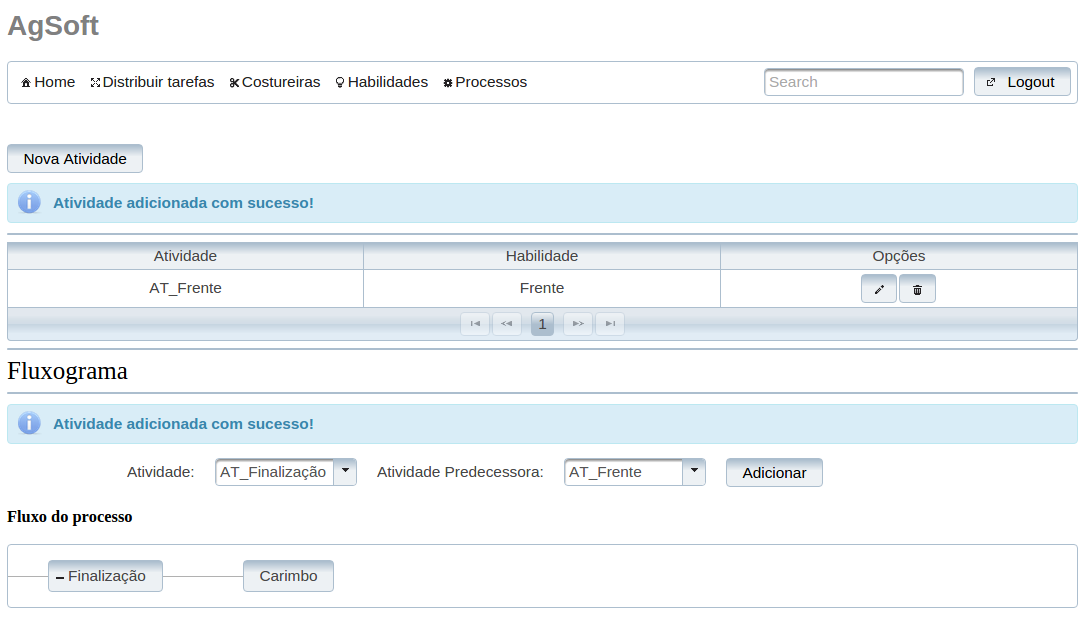
\includegraphics[width=14.7cm]{./imagens/adiconar_atividade_frente_teste5.png}}
	\caption[Adição de uma atividade ao processo.]
	{Adição de uma atividade ao processo. \textbf{Fonte:} Desenvolvido pelos
	autores.}
	\label{fig:add_frente_teste5}
\end{figure}

\par Após a adição da atividade, é preciso adicioná-la ao fluxo do processo como
predecessora da atividade finalização. Como a atividade finalização é sempre a
última atividade do processo, todas as atividades que forem incluídas sempre
serão predecessoras a ela. A Figura~\ref{fig:add_frente_teste4} mostra a atividade frente adicionada
ao fluxo do processo.

\newpage

\begin{figure}[h!]
	\centerline{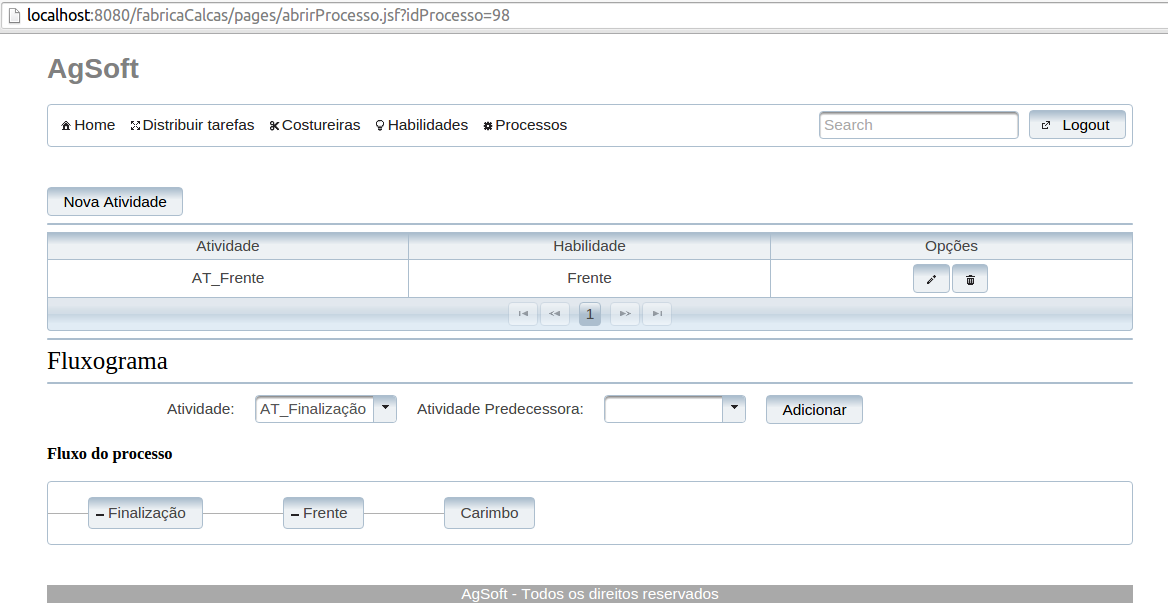
\includegraphics[width=14.7cm]{./imagens/adicionar_atividade_frente_teste4.png}}
	\caption[Adição de uma atividade ao fluxo do processo.]
	{Adição de uma atividade ao fluxo do processo. \textbf{Fonte:} Desenvolvido
	pelos autores.}
	\label{fig:add_frente_teste4}
\end{figure}


\par Foram adicionadas na habilidade frente as costureiras Roberta, Lúcia e
Renata, para que pudessem realizar a atividade frente do processo.
\par A Figura~\ref{fig:add_costureira_frente_teste4} mostra as costureiras
adicionadas na habilidade frente.

\begin{figure}[h!]
	\centerline{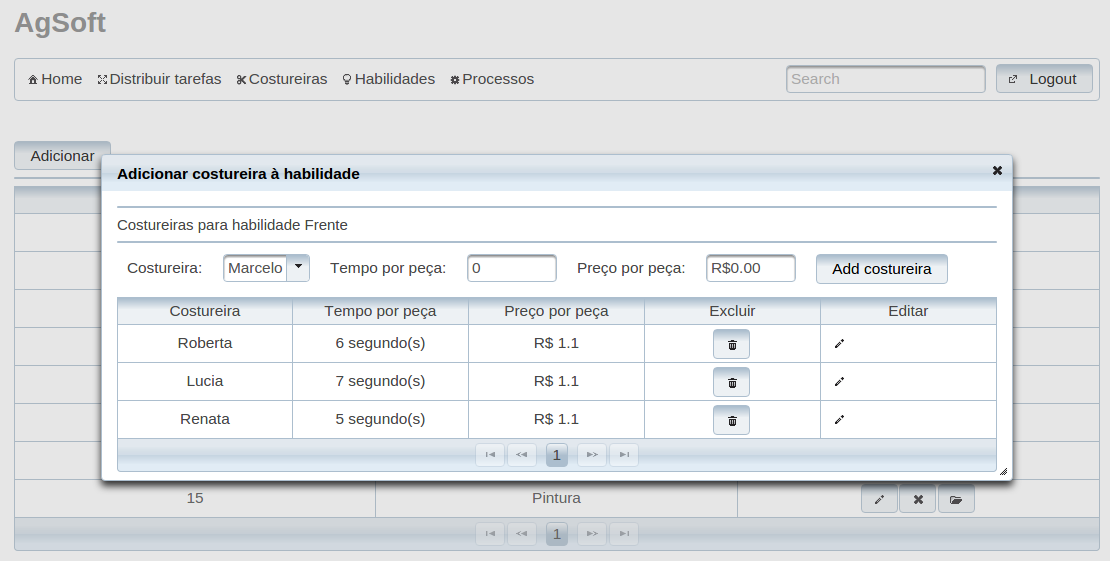
\includegraphics[width=14cm]{./imagens/costureiras_at_frente_tete5.png}}
	\caption[Adição de costureiras na habilidade Frente.]
	{Adição de costureiras na habilidade Frente. \textbf{Fonte:} Desenvolvido pelos
	autores.}
	\label{fig:add_costureira_frente_teste4}
\end{figure}

\par Feito isso, foi realizada a distribuição dos lotes com as configurações de
tempo e custo, mostradas na Figura~\ref{fig:add_costureira_frente_teste4} e com
as informações de localização das costureiras, mostradas na
Figura~\ref{fig:add_xy_costureira_teste4}.
\par A Figura~\ref{fig:resultado1_teste5} mostra o resultado obtido na
distribuição.

\newpage

\begin{figure}[h!]
	\centerline{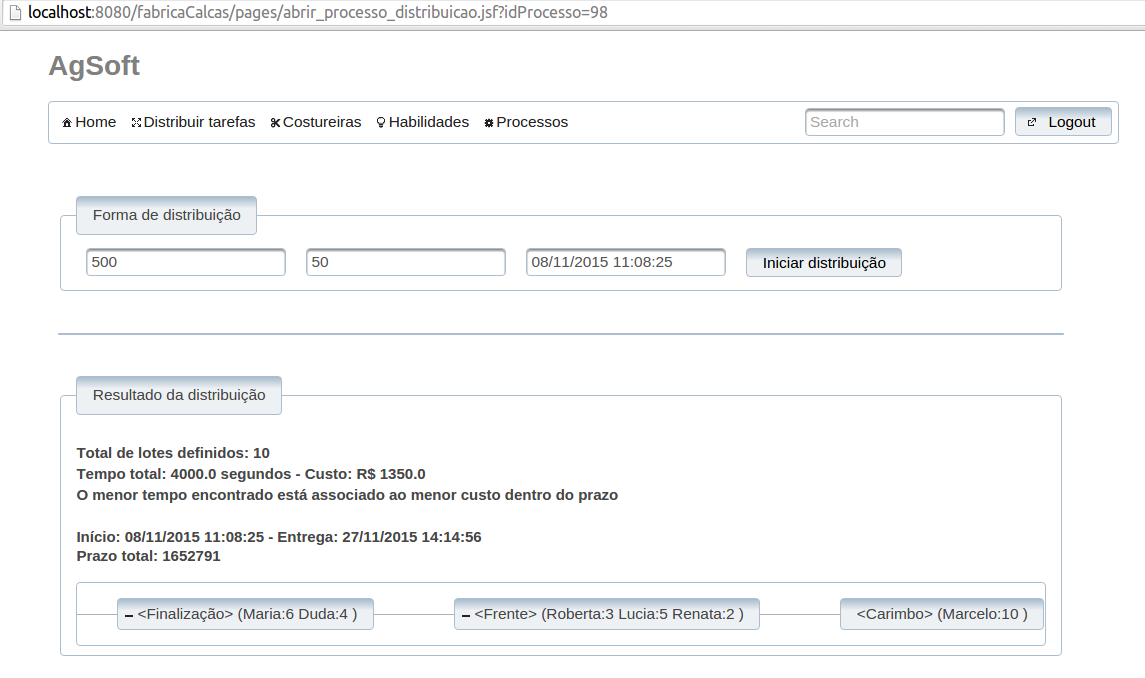
\includegraphics[width=14.7cm]{./imagens/resultado1_teste5.png}}
	\caption[Resultado da distribuição de lotes com mais uma atividade.]
	{Resultado da distribuição de lotes com mais uma atividade. \textbf{Fonte:} Desenvolvido pelos
	autores.}
	\label{fig:resultado1_teste5}
\end{figure}

\par Com base na Figura~\ref{fig:resultado1_teste5}, pode-se observar que foi
adicionada no resultado final a atividade frente e suas respectivas costureiras.

\par A Figura~\ref{fig:detalhamento1_teste5} mostra o detalhamento da
distribuição da Figura~\ref{fig:resultado1_teste5}.


\begin{figure}[h!]
	\centerline{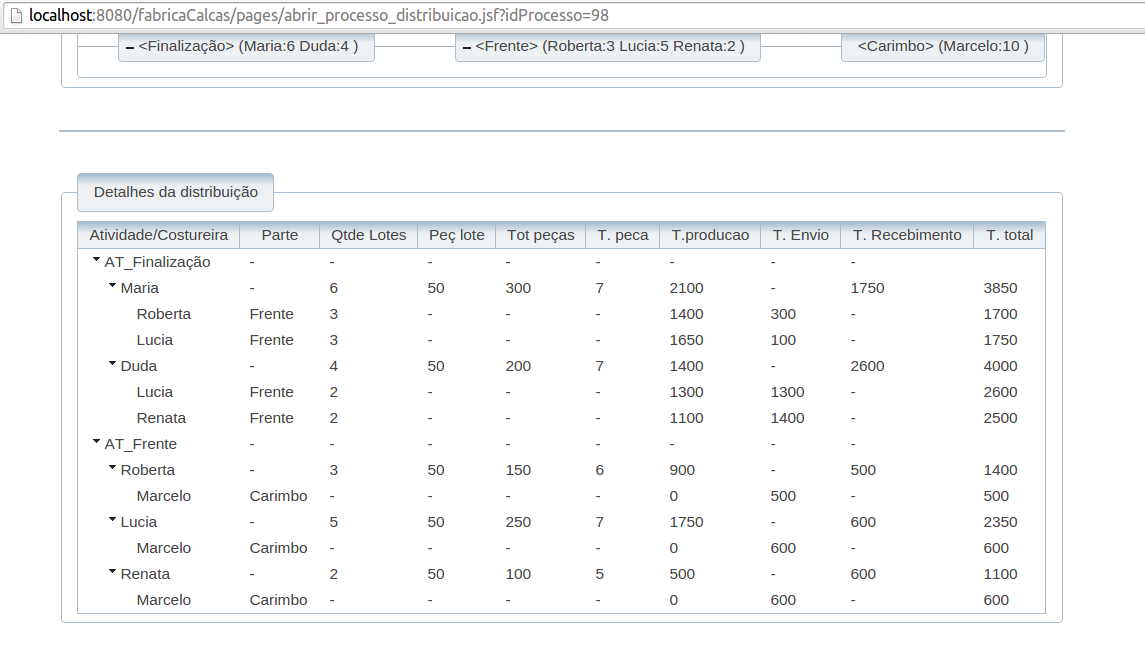
\includegraphics[width=14.7cm]{./imagens/detalhamento1_teste5.png}}
	\caption[Distribuição das atividades.]
	{Distribuição das atividades. \textbf{Fonte:} Desenvolvido pelos
	autores.}
	\label{fig:detalhamento1_teste5}
\end{figure}

\par Vale ressaltar que, ao executar a distribuição, o algoritmo pode
encontrar várias soluções que contêm o mesmo resultado e retornar uma delas. Se
a distribuição for executada novamente mantendo as configurações das costureiras
como a posição X e Y, tempo e custo, a distribuição poderá ocorrer de uma outra
forma, conforme mostra a Figura~\ref{fig:resultado2_teste5}.



\begin{figure}[h!]
	\centerline{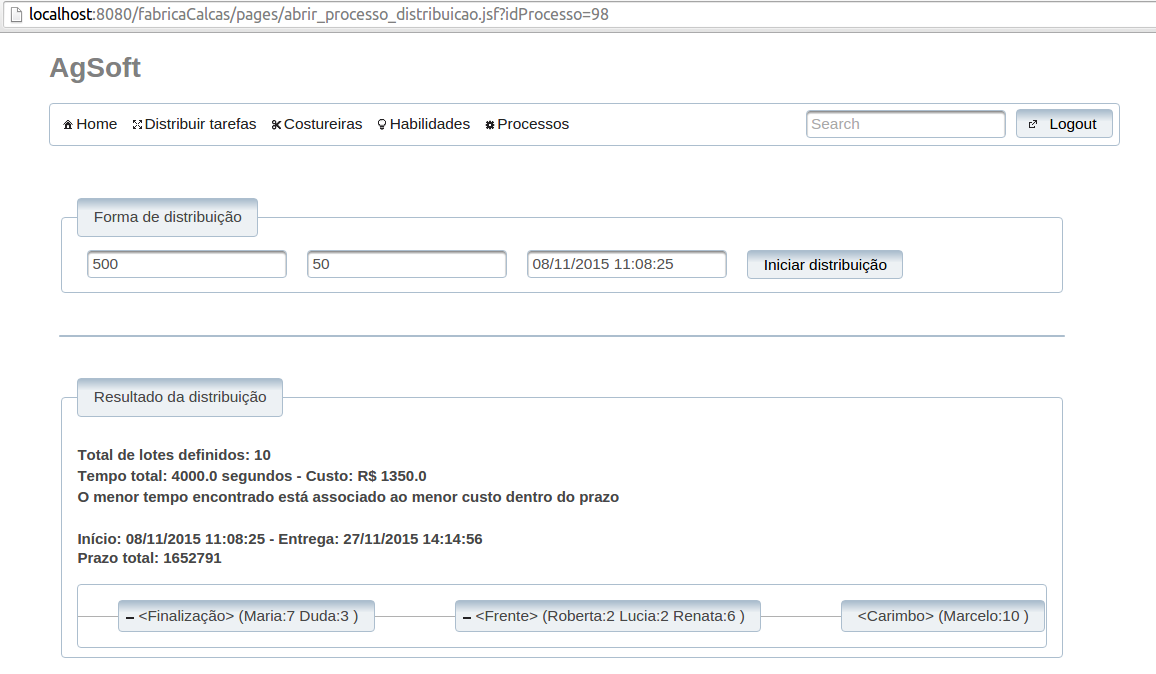
\includegraphics[width=14.7cm]{./imagens/resultado2_teste5.png}}
	\caption[Resultado da distribuição de lotes após executar novamente a
	distribuição.]
	{Resultado da distribuição de lotes após executar novamente a
	distribuição. \textbf{Fonte:} Desenvolvido pelos autores.}
	\label{fig:resultado2_teste5}
\end{figure}


\par A Figura~\ref{fig:detalhamento2_teste5} mostra o detalhamento da
distribuição da Figura~\ref{fig:resultado2_teste5}.

\begin{figure}[h!]
	\centerline{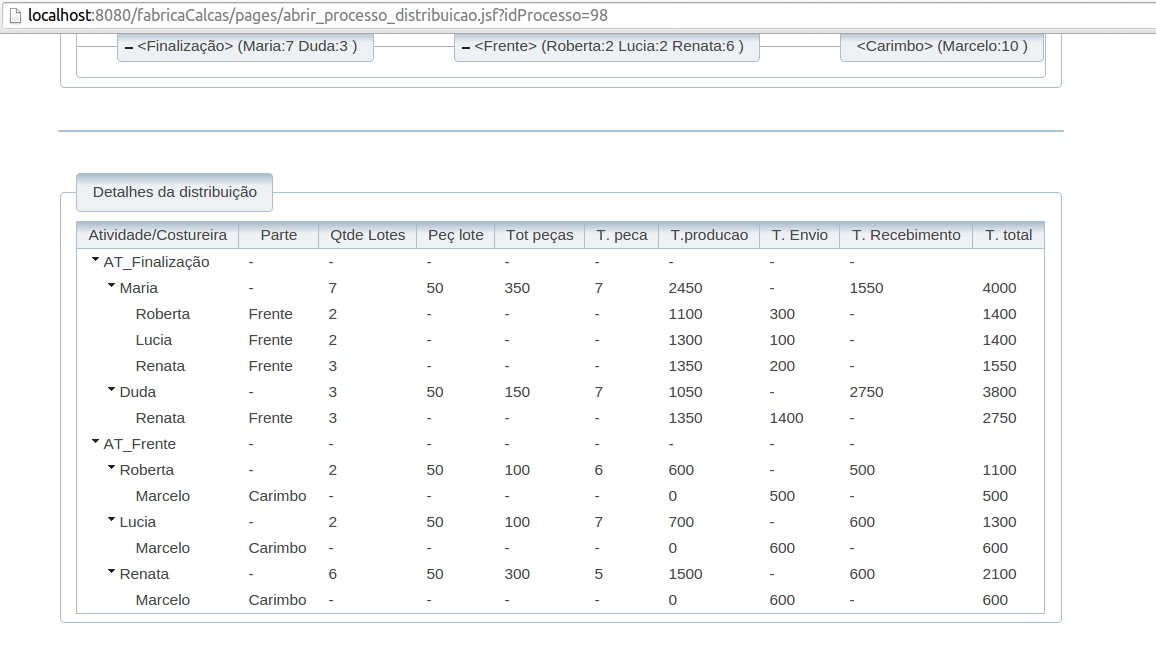
\includegraphics[width=14.7cm]{./imagens/detalhamento2_teste5.png}}
	\caption[Distribuição das atividades.] 
	{Distribuição das atividades. \textbf{Fonte:} Desenvolvido pelos
	autores.}
	\label{fig:detalhamento2_teste5}
\end{figure}


\par Com base nas Figuras~\ref{fig:resultado1_teste5}
e~\ref{fig:resultado2_teste5}, o custo final não teve alterações de uma distribuição para outra, porém 
pode-se observar que o tempo total de produção e o tempo de
distribuição dos lotes entre as costureiras é realizado de uma forma
diferente, concluindo assim que o algoritmo encontrou outra forma de realizar a
distribuição, mantendo o melhor resultado.

\section{Teste quando o prazo não é atendido}

\par Este teste foi realizado para demonstrar quando o prazo de entrega das
peças não consegue ser atendido. Esse teste realiza a distribuição para o mesmo
processo da seção 4.1.

\par A Figura~\ref{fig:configuracao_costureiras_teste6} mostra a configuração
das costureiras da habilidade finalização.

\begin{figure}[h!]
	\centerline{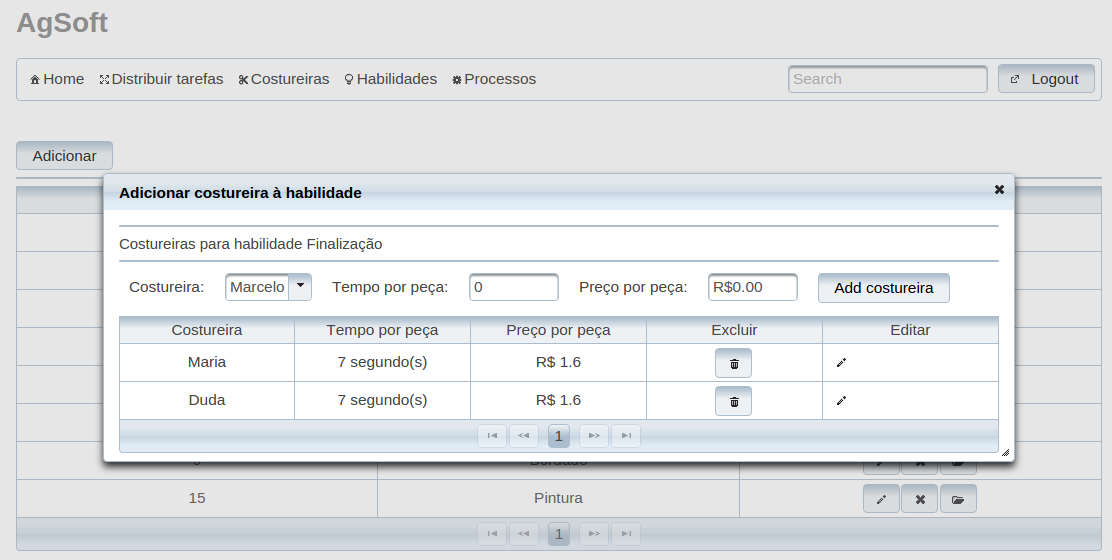
\includegraphics[width=14.7cm]{./imagens/configuracao_costureiras_teste6.png}}
	\caption[Configuração das costureiras da atividade Finalização.] 
	{Configuração das costureiras da atividade Finalização. \textbf{Fonte:} Desenvolvido pelos
	autores.}
	\label{fig:configuracao_costureiras_teste6}
\end{figure}

\par Considerando as configurações mostradas na
Figura~\ref{fig:configuracao_costureiras_teste6}, foi iniciado o processo de
distribuição dos lotes, como mostra a Figura~\ref{fig:resultado1_teste6}.

\begin{figure}[h!]
	\centerline{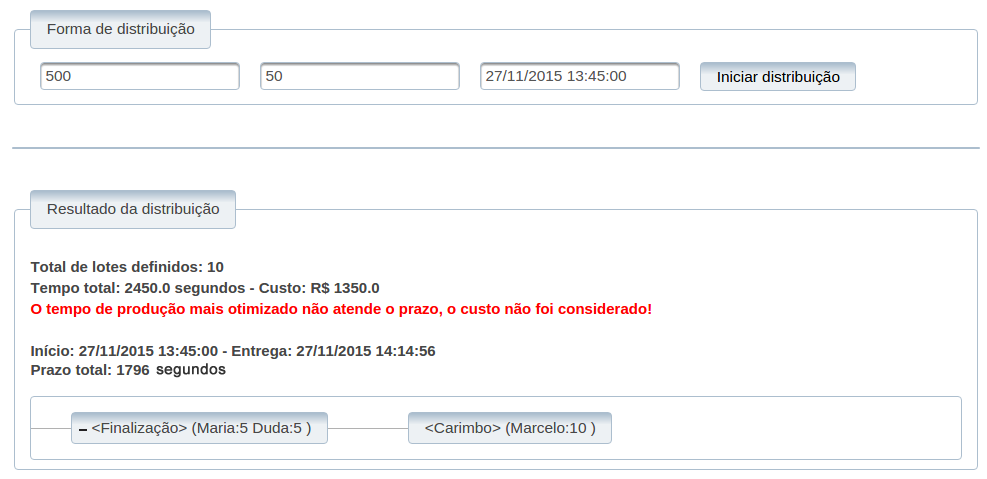
\includegraphics[width=13cm]{./imagens/resultado1_teste6.png}}
	\caption[Resultado da distribuição de lotes com prazo não atendido.] 
	{Resultado da distribuição de lotes com prazo não atendido. \textbf{Fonte:} Desenvolvido pelos
	autores.}
	\label{fig:resultado1_teste6}
\end{figure}

\par Como mostrado na Figura~\ref{fig:resultado1_teste6}, o prazo de produção
é de 1796 segundos e, mesmo alocando todas as costureiras, não foi possível
entregar as peças no prazo determinado, pois o tempo mínimo possível de produção
é de 2450 segundos. O algoritmo foi desenvolvido para manter sempre o menor custo, procurando manter o tempo
dentro do prazo, porém caso nenhum dos indivíduos tenha o tempo total menor que o prazo,
então o melhor tempo é retornado e o custo é desconsiderado.
Para demonstrar isso, foi alterado o custo da costureira Duda, conforme mostra a
Figura~\ref{fig:alterecao_custotcseis}.
 

\begin{figure}[h!]
	\centerline{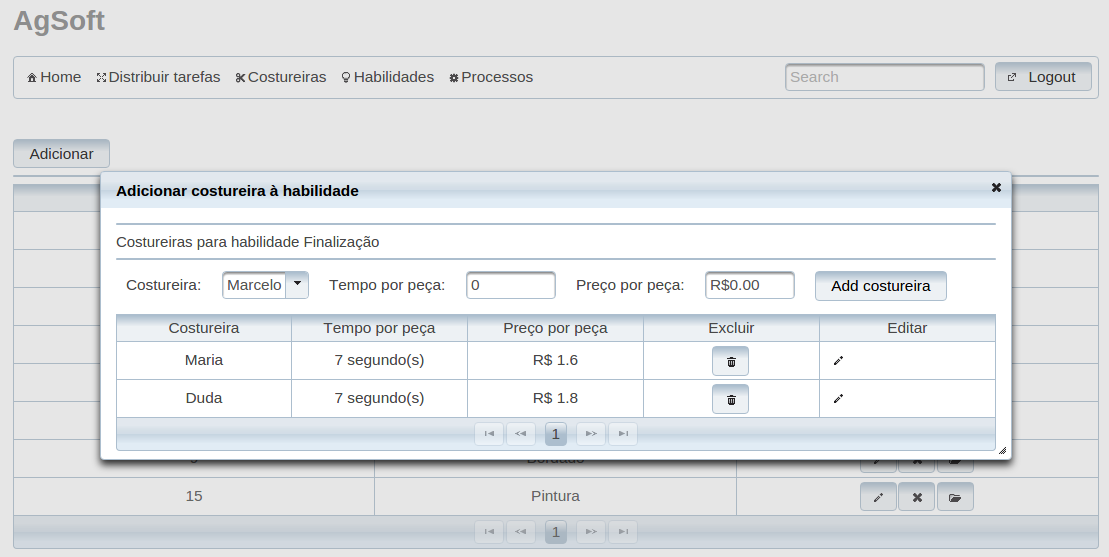
\includegraphics[width=14.7cm]{./imagens/alterecao_custo_teste6.png}}
	\caption[Alteração no custo das costureiras da habilidade Finalização.] 
	{Alteração no custo das costureiras da habilidade Finalização. \textbf{Fonte:} Desenvolvido pelos
		autores.}
	\label{fig:alterecao_custotcseis}
\end{figure}

\par Foi iniciada novamente a distribuição dos lotes, conforme mostra a
Figura~\ref{fig:resultado2_teste6}.

\begin{figure}[h!]
	\centerline{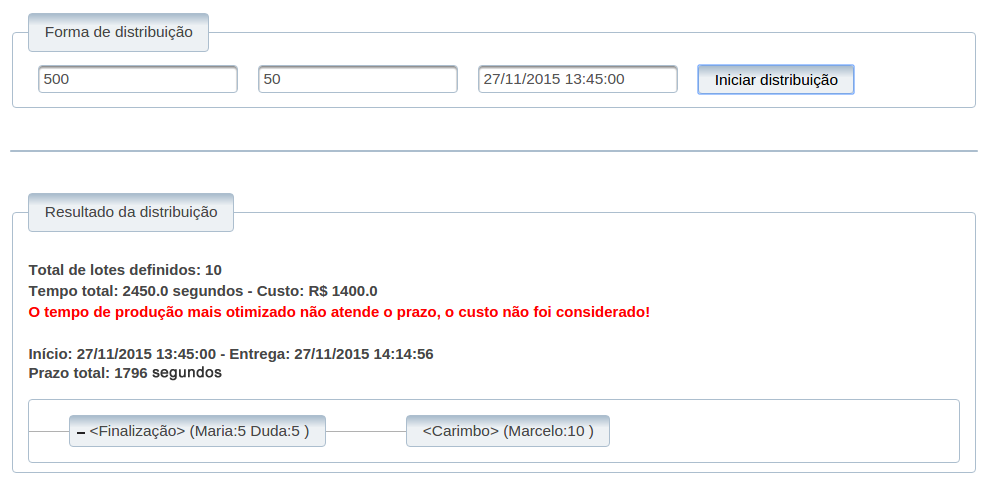
\includegraphics[width=14.7cm]{./imagens/resultado2_teste6.png}}
	\caption[Resultado da distribuição após alteração no custo da costureira Duda.] 
	{Resultado da distribuição após alteração no custo da costureira Duda. \textbf{Fonte:} Desenvolvido pelos
	autores.}
	\label{fig:resultado2_teste6}
\end{figure}

\par Conforme mostrado na Figura~\ref{fig:resultado2_teste6}, mesmo com o
aumento no custo por peça da costureira Duda, o algoritmo ainda assim distribuiu
lotes para esta costureira, aumentando o custo final, porém retornou o
menor tempo de produção possível.
